\documentclass{article}
\usepackage[utf8]{inputenc}
\usepackage[english]{babel}
\usepackage[document]{ragged2e}

\usepackage[sorting=none]{biblatex}
\addbibresource{references.bib}

%\usepackage{url}
%\usepackage[numbers]{natbib}
\usepackage{indentfirst}
\usepackage{graphicx}
\usepackage{geometry}
\usepackage{listings}
\usepackage{float}
\usepackage{hyperref}
%\hypersetup{
%    colorlinks=true,
%    linkcolor=blue,
%    filecolor=magenta,      
%    urlcolor=cyan,
%}


\begin{document}

\title{Blockchain based investment cooperative application}
\author{\IEEEauthorblockN{Mubarak Mikail, Sam Seneza}\\
\IEEEauthorblockA{\textit{College of Engineering} \\
\textit{Carnegie Mellon University Africa}\\
Kigali, Rwanda \\
\{mmikail, sseneza\}@andrew.cmu.edu}
}
\date{February 2020}

\maketitle

%\tableofcontents
\begin{flushleft}
\section{Abstract}

\section{Introduction}
The number and size of cooperatives around the world keeps increasing day-by-day which also goes with the rise in the amount of money that is being contributed, and along this is an increased need for strong and reliable management of these cooperatives. Book-keeping, safekeeping, and the security of the circulation and the use of this cooperative money gets more and more tedious. With this need in mind, one would start to think about ways of solving and strengthening the cooperative work system in general. This paper looks into how cooperative operations and processes can be made simpler and more secure with the blockchain technology. The blockchain technology is simply a data structure used for storing data, more formally, which can be regarded as an open distributed ledger which stores transactional data in a way that is permanent and persistent i.e., that is they cannot be edited or modified once they are on the blockchain. In addition to this, every transaction that is recorded on the blockchain is known to all parties involved, hence there is no form of mystery involved in the transactions as each and every transaction is made publicly available. These transactions are kept in a distributed ledger that can be verified without the need of a trusted third-party to verify the transaction details and these transactions are kept irrevocably permanent. \cite{alma991019600567904436}

\subsection{Background of the Project}
Cooperative contribution involves a group of people coming together to pull some money together on either a monthly, quarterly or yearly basis and at the end of that period, one person takes all the money, another person in the group takes the one for the next period and it goes on like that until everyone gets their fair share before the cycle comes back to continuity. This functioning cooperative is set in order to raise funds to help its members to get increased access to monetary resources without the hassle of requesting loans from banks. This implies that members can also request for loans from the cooperative and would have to pay back after a certain period of time with some additional charges.

Cooperative contributions may be highly beneficial to its members and these operations have been around for a long time, in fact, cooperative saving and credit institutions can be traced back in the 19th century especially in Germany where there was a credit cooperative for minor artisans and the urban middle classes \cite{galor2018saving}. These types of cooperatives are basically put in place to avoid the difficulties of obtaining credit from a bank or another financial institution. The cooperative members help each other to prevent poverty with mutual aid and self-reliance. Members are encouraged to contribute money, and this money enables them to receive loans from their accumulated savings for various reasons. The benefits of cooperatives are not only reaped by the loan seekers, they are reaped by everyone because whenever one of the members takes a loan, they repay the money with some interest that can be shared among the cooperative members. Cooperative contribution can in some ways also be a safeguard to money of the parties involved since the cumulative amount can be shielded in advantage over time. \cite{galor2018saving}

In cases where a member gets money from the cooperative, the factors influencing repayment vary depending on interest rates, the duration of loans, personal sources of income, and much more \cite{papias2009repayment}. This may raise the uncertainty of member’s money safety. Bookkeeping of the cooperative’s money may be exasperating, and ways to misuse the money may arise from the process.

\subsection{Problem Statement}
Cooperatives may be operating in slightly different ways, but besides that, in our case we drill down on the contribution cooperative approach i.e., members contribute collectively and then choose one of them to take all the money (or a certain amount agreed on by all members) in the cooperative. This person may use the money in a variety of their own projects and is expected to pay back after a certain period of time with a set interest depending on the agreement. This cooperative money in some cases may be highly controlled by the cooperative president \cite{nilsson2013cooperative}.

Digging deeper into the current cooperative functioning system, a cooperative president who may have some superior control over the cooperative money may decide to misuse these funds. A person may get to be selected to take the money cyclically with some bias. A person who takes/borrows the money may, with little or no difficulties, erase the traces that they are in a temporal possession of the money. These kinds of problems do occur especially with the non-transparent decision-making process within cooperatives, limited managerial or leadership capacities by some members, and external help in connection with the cooperative's development \cite{rca001}. This problem could be stated generally as the misuse of cooperative funds as this non-transparency mostly suggests.

This misuse of cooperative money problem could be addressed with the introduction of a distributed ledger technology, that is a digital decentralized solution to be employed as a smart way to mitigate this kind of problems, in other words, employing the blockchain technology in order to address the problem of some privileged members to misuse the funds as each and every transaction would be stored permanently and irreversibly in the system. This would make the exchange of information regarding the movement of money easy and with more clarity \cite{rodrigues2019evaluating}.

\subsection{Area of Focus}
A functioning cooperative is set up in order to raise funds to help its members to get increased and fast access to monetary resources without the bottlenecks involved in requesting loans from banks. This cooperative system is designed and agreed on by cooperative members that are willing to join and due to this fact, some people may think that when choosing who should take the money there is some bias (which may also be true in some cases). And if this can happen, it suggests that the system may need some improvements. What if there was a digital system to randomly select one person, that person then becomes the one assigned to take the money for their use, and then that system removes that person from the possibility to be randomly selected before the cycle restarts. In other words, once a person is selected, they are removed from the choices within the same cycle, but they are to be brought again after the cycle ends hence ensuring that no person is selected to get the money twice within one cycle.

In the current traditional method of managing cooperative activities, a third party watcher may have to be involved in order to ensure smooth and trusted operations \cite{nair2018blockchain}. An improvement here would be bringing in blockchain to record cooperative members’ contributions with a specialty of being publicly verifiable \cite{nair2018blockchain}. And in addition to that, an unbiased algorithm to select who should take the money at a certain point in the cycle would be incorporated into the technology therefore improving the reliability of the cooperative functioning. 

\section{Literature Review}
A cooperative is basically a firm that is set up by a group of people to serve for collective benefit. They contribute monetary resources together so that they can share and meet specific target objectives. Generally within cooperatives, people can also get loans usually at smaller interest rates compared to regular financial situations. A cooperative can also be referred to as a business organization with limited liability where each shareholder has one vote regardless of the shares they own \cite{credo22393191}. The advantages of a cooperative functions are expressed as an organization that is operated for the benefits of the people using its services that may be mostly its members \cite{credo17700186}.

Cooperative work's efficiency may be improved by solving extensively some of its current major problems and some of those current problems are listed below \cite{rca001}:
\begin{enumerate}
    \item The capacity of cooperative leadership and management.
    \item Lack of democratic control by the members.
    \item Third party involvement which could lead to collusion, theft and fraud.
\end{enumerate} 

These problems stated above are imperceptibly contrary i.e., are equivalent to our mainly identified problem of the tendency of misusing cooperative funds as discussed in the statement of the specific problem to be addressed. 

A recent study of 450 cooperatives in Tanzania and Sri Lanka reports that cooperatives lack access to loan finance to help them expand their business. 
 
“Equality is one of major guiding values of cooperatives. An open and voluntary membership is one of the principles to which cooperatives hold dear. Cooperative enterprises prefer to have a “one member, one vote” system, which ensures that decision making powers are equally distributed amongst the members . Cooperatives are people-centric enterprises, hence they end to focus on the needs of their members and of the communities in which they operate, rather than on financial returns alone.” \cite{un_issues} This is related to the second problem stated above.

Regarding the capacity of the cooperative leadership and management, and the lack of democratic control by the members of a cooperative can lead to the doom of their endeavors. Research has found that the growth of these kinds of organizations may be facilitated by relying on blockchain technology as their source of distributed governance or control. \cite{mannan2018fostering}

Another research has also spotted a potential means to the improvement of cooperative leadership and management. This specifically is the transparent and available bookkeeping where it was stated that the blockchain technology can be of great importance in improving the bookkeeping methods of Kenyan cooperatives basically because all activities would be transparent and available to everyone anytime. \cite{mitch_national}

A proposal in a research suggests a blockchain federated intermediary architecture in order to help everyday cooperation activities. This proposal goes a step further showing the benefits that could be witnessed by a number of cooperatives with heterogeneous information i.e., separated information if all cooperative chains' information was now made easy to be traversed. \cite{ieee_s8637578} 

Research has shown that blockchain can be used as a data sharing platform for cooperative purposes while ensuring its overall security, and also most importantly ensuring its traceability towards the satisfaction off human needs in cooperatives. \cite{alma991019580288704436, proquest2282979983} 

Primarily, we are trying to solve this possibility of funds misuse as specified above by ensuring transparent cooperative leadership and transactions. Blockchain can help us with tackling the challenges of lack of democratic control among the members and third party involvement in the cooperative activities which usually have detrimental effects on the society.
Not a lot of work has been done prior to this time in this regard though research has highlighted and addressed most of these problems and how they can be resolved by a blockchain network. This implies that transparency in everyday cooperative activities could be fortified towards the mitigation of the problem of misusing funds in cooperatives.

This new system is trying to address these problems stated above, as from empirical research were they found. This system will incorporate the blockchain technology in everyday transactions of cooperatives, set out from contribution to sharing, returning the cooperative money with collective clarity.

\section{Proposed Solution}
A problem is well addressed with a solution. In our case, there has been identified a problem in cooperatives regarding the misuse of funds. While addressing this problem, a solution of a blockchain network with a distributed ledger technology is proposed.

The goal of this solution is to make easy the cooperative contribution record-keeping system currently done manually by members. Our proposed solution is a decentralized application that is going to employ a DLT (Distributed Ledger Technology) which is a distributed non-repudiatory way in keeping track of the amount of money each member of the group is contributing to the wallet i.e., contributions should be recorded trace by trace permanently. Unlike current systems where there are issues when it comes to determining who gets paid for each period as people might not be very comfortable with them not getting their share early in the contribution stages. 

In addition to this, the problems regarding the possibility of bias in the selection of who to receive the money at a certain period would be eliminated with a digital system that would purely select randomly which of the members is to receive the money. An algorithm will be employed to select recipients of the general contribution for each period, this will bring some trust to this group. The algorithm will involve assigning unique ids to each member of the cooperative such that at the end of each period that is at the time of collections, a unique id will be selected from that pool by the computer and the owner of that id gets the contributions for that period, this id is then taken out of the pool. This will be iterated every period end.

This solution can be extended to investments in other cryptocurrencies and other commodities in the near future. An individual can also choose to use it to save money over a period. The DLT is there to show the amount everyone is contributing, there is fairness and trust as everyone involved will have access to this data. There are certain challenges that might be associated with this solution, however we will look at how to mitigate these challenges.

\begin{figure}[H]
\centering
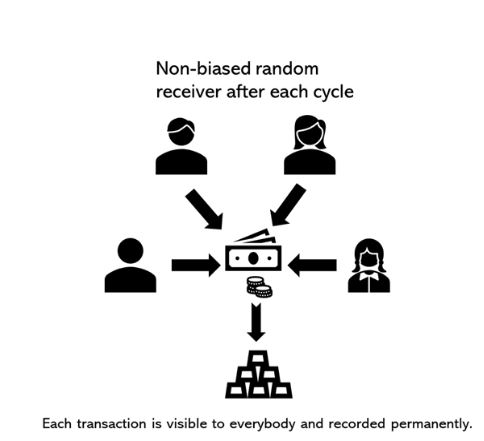
\includegraphics[scale=1.0]{cop}
\caption{Overview of the proposed solution}
\label{fig:central}
\end{figure}

\section{Methodology}
This solution is going to be implemented in 2 main parts:
\begin{enumerate}
    \item General algorithm for the decentralized application
    \item Algorithm for selecting which of the members gets paid at the end of the period.
\end{enumerate}

The selection of who gets paid has been discussed in the previous section on proposed solution \& algorithm. Here, we will talk more about a general algorithm for implementing our application. Much of the coding of our smart contract is going to be done in Solidity. Two major contracts will be implemented with solidity. We will start by creating a contract in solidity that will represent the cooperative group. This contract will abstract away certain features of a cooperative and functions we want our cooperative to be able to perform. The other contract will be the member contract, it will encapsulate behaviors that will be expected of the members of a cooperative and each member will have a means of identification on the blockchain which is going to be their address. This will be generated off the Ethereum Blockchain. Each member will have their own address and there is going to be an address for the cooperative pool also such that all the members of the cooperative can pay to that address and we can see the balance and transactions occurring on that address at any given point in time.
Some of the deliverables we hope to achieve at the end of this project are:
\begin{itemize}
    \item A working decentralized application.
    \item A group of people should be able to come together and form a cooperative on this App.
    \item They should also be able to send money to a particular address.
    \item All transactions to this address must be visible to everyone in the group especially.
    \item We aim to implement this solution as a web application.
\end{itemize}

The members of a cooperative will be able to perform the following actions:
\begin{itemize}
    \item Send digital money to the cooperative pool.
    \item Check the amount they have left based on their address. They can only check their own balance.
    \item Members can only send money if they have to up to that amount in that wallet. If they don't have up to that amount in their wallet, the transaction should not go through.
    \item Set address to be paid to.
    \item Show the current address that is being paid to.
\end{itemize}

The cooperative pool will be able to perform the following actions:
\begin{itemize}
    \item Send money to one unique member at the end of each month.
    \item Ensure not to pay a member that has been paid before until every other member of the cooperative has been paid.
    \item Keep track of the addresses being paid and the value paid into those addresses.
    \item Take every address that has been paid out of the pool to be paid temporarily.
    \item Check the balance left on the pool.
    \item Set address to be paid to.
    \item Show the current address that is being paid to.
\end{itemize}

\subsection{Tools and Datasets}
This solution is going to ride on Ethereum as the main blockchain technology. Most decentralized applications run on Ethereum. Ethereum has two main components: Smart contracts and Distributed Ledger Technology (DLT), they will be very important in this implementation. On Ethereum, applications that can control digital value and are accessible from any part of the world can be implemented. Solidity and JavaScript will be used to build the application. \href{https://remix.ethereum.org/}{Remix IDE} will be used to write and compile our Solidity program. For testing purposes, this solution can be deployed on Remix such that its functionalities can be tested. Another testing tool that can be used for this solution is Truffle Ganache, a web3 provider application which is available across the major platforms, Windows, Mac OS X and Linux. Infura is another service that can be used to deploy our Blockchain solution. \cite{czombies} Infura is a service that maintains a set of Ethereum nodes with a caching layer for fast reads, which you can access for free through their API. Using Infura as a provider, you can reliably send and receive messages to and from the Ethereum blockchain without needing to set up and maintain your own node. A chrome extension called MetaMask could also be used for deployment and testing, it rides on an injected web3 environment.\cite{czombies} Metamask is a browser extension for Chrome and Firefox that lets users securely manage their Ethereum accounts and private keys, and use these accounts to interact with websites that are using Web3.js. By installing MetaMask, your browser is Web3 enabled and you would have the ability to interact with any website that communicates with the Ethereum blockchain!). For testing, we decided to stick with the JavaScript virtual machine on Remix website. This has the advantage of being in the same environment as the compiler and development environment, hence it is more convenient.

\begin{figure}[H]
\centering
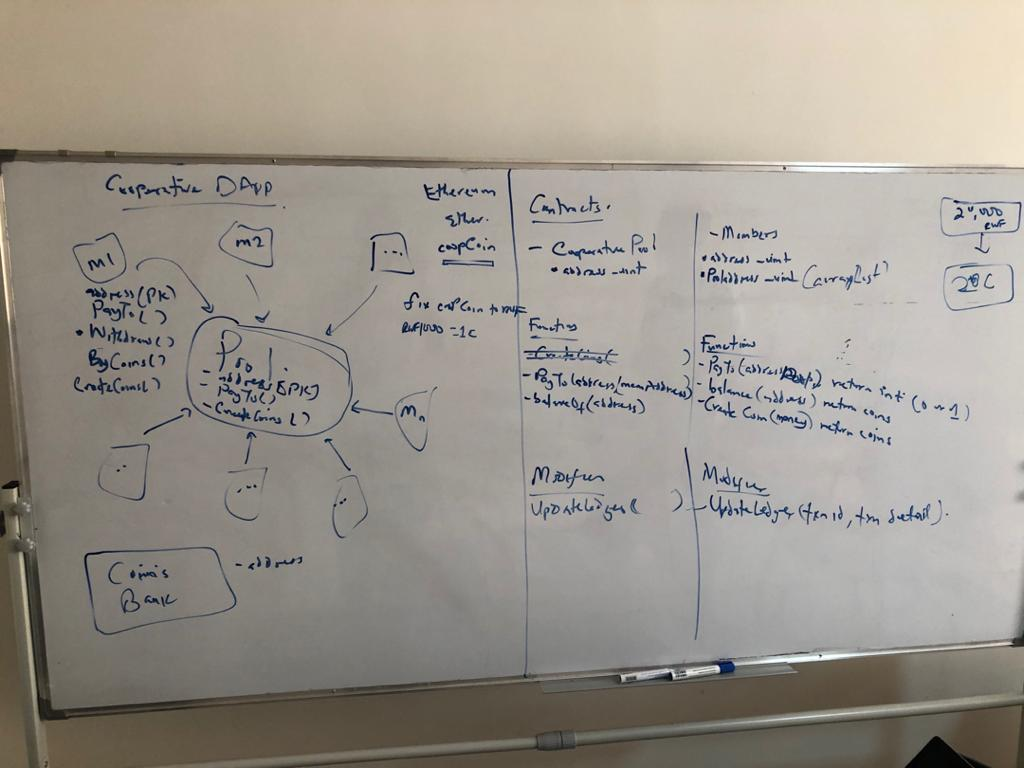
\includegraphics[scale=0.4]{design}
\caption{Blackboard sketch of the design}
\label{fig:dessign}
\end{figure}

\begin{figure}[H]
\centering
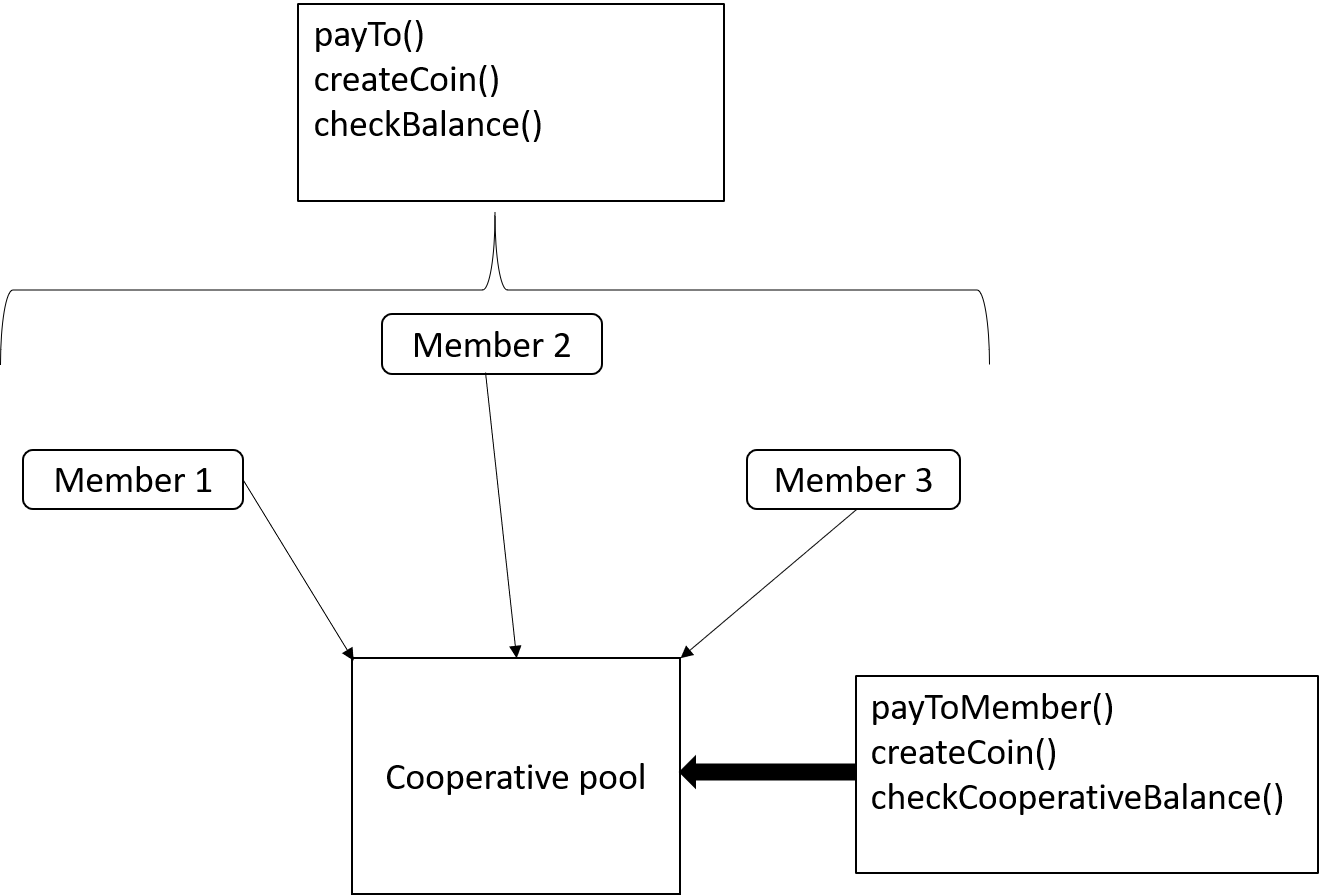
\includegraphics[scale=0.4]{KeyFunct.png}
\caption{Illustration of key functionalities of the application}
\label{fig:dessign}
\end{figure}

\section{Implementation}
The blackboard sketch of our design is shown in Fig. 2. We are modelling our design in a way such that we have basically two(2) main contracts. A member contract where we are trying to abstract away all the details and functions of members in the cooperative. The other contract is the cooperative pool contract, here we have the details of the pool where the members will be transferring their contributions to. In the cooperative pool contract we also have functions that we want the pool to be able to perform. 

Certain behaviors are common to both contracts, these  include: payTo() function, a mapping that can be used to link addresses to integer value which will represent the balance of the contract. Both contracts have get and set functions for the addresses to be payed into since address of the receiver is set as an instance payable variable in the contracts. There is a constructor that is used to initialize the contract with an address. A modifier was also added to these contracts for security purposes in order to ensure that only the addresses related to these contracts can call the functions under the contract. Our get functions were implemented as a view since we are not going to be making any changes to any variable in the contract and to save gas costs which translates to Ether. Code optimization is more important in Solidity than any other programming language. The codes for this project can be found on Github through the link: \url{https://github.com/e-mubaraq/coop-DApp}

\section{Results and Discussion}
Some of the results we wish to achieve from this implementation include:
\begin{itemize}
    \item Successfully set up a contract for members
    \item Successfully set up a cooperative pool contract
    \item Ability to make transfers between these two contracts
    \item Ability to see the balance left on these contracts
\end{itemize}
We have been able to develop a solution that simulates the parties involved in a cooperative society and how they interact with each other. At the very basic level, they should be able to transfer money to each other which is represented in the form of digital cash in our Blockchain solution. We are still working on implementing the randomization algorithm that allows the cooperative pool to pick which member gets paid at he end of the period and ensuring that this member doesn't get doubly paid while the rest are yet to get any remittance from the pool.

\section{Conclusion}
One of the major problem currently associated with the traditional cooperative society is the mismanagement of funds which is associated with the presence of a third party that accepts payment from the members, our blockchain cooperative pool  solves this particular problem as it is decentralized and everyone can see what is going on in the pool at every point in time.

This solution could be adapted into investments and stocks management in the future. The ground work has been laid out already in our code. Some additional functionalities will be added to this code to enable it perform this new functions. This is just a few among the solutions it could be adapted to in the future and we will try to be available to work with anyone who wants to build on top of our solution. Another implementation that could be added in the future is perfecting the randomness of member selection for payment at the end of each contribution period.

\cite{deloitte} A publication by Deloitte also enforces the opportunity for Blockchain applications in investment management due to certain features of the Blockchain like the fact that there is a digital identity associated with each individual which is linked to their financial record and transactional history.

\end{flushleft}
%\bibliographystyle{ieeetr}
%\bibliography{references}

\clearpage
\printbibliography

\end{document}
